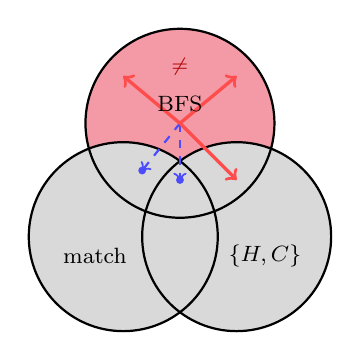
\begin{tikzpicture}[scale=1.2]
  % Define the circles - all same size, arranged in triangle
  \def\circleRadius{1cm}
  \def\offset{0.6cm}
  
  \begin{scope}[blend group=multiply]
    % BFS circle - top
    \fill[blue!30, opacity=0.5] (0,\offset) circle (\circleRadius);
    % match circle - bottom left
    \fill[yellow!40, opacity=0.5] (-\offset,-\offset) circle (\circleRadius);
    % {H, C} circle - bottom right
    \fill[green!30, opacity=0.5] (\offset,-\offset) circle (\circleRadius);
  \end{scope}
  
  % Highlight the region: BFS \ (match ∪ {H,C})
  % This is BFS excluding both match and {H,C}
  \begin{scope}
    \clip (0,\offset) circle (\circleRadius);
    \fill[red!50, opacity=0.7] (-3,-3) rectangle (3,3);
  \end{scope}
  % Now cut out the match circle
  \begin{scope}
    \clip (-\offset,-\offset) circle (\circleRadius);
    \fill[gray!30, opacity=1] (-3,-3) rectangle (3,3);
  \end{scope}
  % Now cut out the {H,C} circle
  \begin{scope}
    \clip (\offset,-\offset) circle (\circleRadius);
    \fill[gray!30, opacity=1] (-3,-3) rectangle (3,3);
  \end{scope}
  
  % Draw circle outlines
  \draw[thick] (0,\offset) circle (\circleRadius);
  \draw[thick] (-\offset,-\offset) circle (\circleRadius);
  \draw[thick] (\offset,-\offset) circle (\circleRadius);
  
  % BFS search arrows - showing search propagating outward
  % Arrows that stop at match boundary
  \draw[->, thick, blue!70, dashed] (0,\offset) -- (-0.4,0.1);
  \draw[->, thick, blue!70, dashed] (0,\offset) -- (0,0);
  % Arrow that continues beyond (into heteroatom region)
  \draw[->, thick, red!70, line width=1.2pt] (0,\offset) -- (-0.6,1.1);
  \draw[->, thick, red!70, line width=1.2pt] (0,\offset) -- (0.6,1.1);
  \draw[->, thick, red!70, line width=1.2pt] (0,\offset) -- (0.6,0);
  
  % Stop markers where BFS hits match
  \node[fill=blue!70, circle, inner sep=1pt] at (-0.4,0.1) {};
  \node[fill=blue!70, circle, inner sep=1pt] at (0,0) {};
  
  % Labels
  \node at (0,0.8) {\footnotesize BFS};
  \node at (-0.9,-0.8){\footnotesize match};
  \node at (0.9,-0.8) {\footnotesize $\{H, C\}$};
  
  % Highlight the target region
  \node[red!70!black, font=\scriptsize] at (0,1.2) {$\neq \varnothing$};
\end{tikzpicture}
